\documentclass[final,a4paper,10pt,abstracton]{scrreprt}

%_DRAFT\usepackage{draftwatermark}\SetWatermarkScale{5}

% This and that
%------------------
\usepackage{etex} % use the etex engine, more variables etc.
\usepackage[utf8]{inputenc}
\usepackage{cmap}    % Correct encoding for Umlaute in pdf
\usepackage[T1]{fontenc}    % Correct hyphenation for non-ASCII characters
\usepackage[english]{babel}
\usepackage{calc}
\usepackage[left]{eurosym}
\usepackage{thumbpdf}
\usepackage{cite} % Order citations automatically (such as [1-4,5,8])
\usepackage{array} % Extend array and tabular with column formatting
\usepackage{hyperref}
\usepackage{textcomp}
\hypersetup{final,
	        plainpages=false,
	        pdfpagelabels,
	        pagebackref,
	        %hyperfootnotes=false,
	        colorlinks=true,
	        linkcolor=blue,
	        urlcolor=red,
	        citecolor=blue,
	        pdfpagemode=UseOutlines,
	        pdfstartview=FitH,
	        pdfborder={0 0 0}}
\usepackage{url}
\usepackage[per-mode=symbol,bracket-unit-denominator=false,detect-all,load-configurations=binary,binary-units]{siunitx}
\DeclareSIUnit\loc{LOC}
\DeclareSIUnit\permil{\textperthousand}

\providecommand{\todo}[1]{{\Large TODO: #1}}
\providecommand{\newterm}[1]{\emph{#1}}
\providecommand{\indexed}[1]{\index{#1}#1}
\providecommand{\product}[1]{{\scshape #1}\index{#1@\textsc{#1}}}
\newcommand{\HRule}{\rule{\linewidth}{0.5mm}}
\newcommand{\ie}{i.\,e.\ }
\newcommand{\eg}{e.\,g.\ }
\newcommand{\cf}{cf.\ }
\newcommand{\dotfillbox}[1]{\makebox[#1]{\dotfill}}


% Tables
%-------------
\usepackage{tabularx}
\usepackage{longtable}
\usepackage{ltxtable}

% Split a cell into multiple rows/columns 
\usepackage{multicol}
\usepackage{multirow}

%\usepackage{slashbox} % Diagonal cells
\usepackage{booktabs}
\usepackage{rotating}


% Graphics
%--------------
\usepackage[all]{xy}
\usepackage{xcolor}
\definecolor{light}{gray}{0.8}
\definecolor{tuerkis}{cmyk}{0.5,0.15,0,0.3}
\usepackage{graphicx}
\usepackage{tikz}
\usetikzlibrary{arrows,positioning,shapes,topaths,calc,fit,backgrounds,matrix,shadows,automata,patterns,decorations.pathmorphing,decorations.pathreplacing,decorations.text,circuits.logic.US,trees,mindmap}
\usepackage{gnuplot-lua-tikz} % GNUplot plots


% Math
%--------
\usepackage{amsmath,amssymb,amstext,amsthm,amsfonts}
%\usepackage{dsfont} %Font for nice set symbols (R, N, Z, ...)
\usepackage{nicefrac} %"Marktfrauenbruch"
% Set symbols
\newcommand{\R}{\ensuremath{\mathds{R}}}
\renewcommand{\P}{\ensuremath{\mathds{P}}}
\newcommand{\N}{\ensuremath{\mathds{N}}}
\newcommand{\Z}{\ensuremath{\mathds{Z}}}
\newcommand{\Q}{\ensuremath{\mathds{Q}}}
\newcommand{\F}{\ensuremath{\mathds{F}}}
\newcommand{\C}{\ensuremath{\mathds{C}}}
% Operators
\newcommand{\entspricht}{\ensuremath{\mathrel{\widehat{=}}}} % entspricht
\providecommand{\abs}[1]{\left\lvert #1 \right\rvert} % Betrag
\providecommand{\norm}[1]{\left\lVert #1 \right\rVert} % Norm
\providecommand{\floor}[1]{\left\lfloor #1 \right\rfloor}   
\providecommand{\ceil}[1]{\left\lceil #1 \right\rceil}   
\providecommand{\svert}{\; \vert \;} %Single vertical bar
\DeclareMathOperator{\grad}{grad} % Gradient
\DeclareMathOperator{\rot}{rot} % Rotation
\DeclareMathOperator{\Div}{div} % Divergenz
\DeclareMathOperator{\rg}{rg} % Rang
\DeclareMathOperator{\Grad}{Grad} % Grad (eines Polynoms)
\DeclareMathOperator{\Abb}{Abb} % Abbildungsmenge
\DeclareMathOperator{\Sym}{Sym} % Bijektionenmenge
\DeclareMathOperator{\Hom}{Hom} % Homomorphismenmenge
\DeclareMathOperator{\End}{End} % Endomorphismenmenge
\DeclareMathOperator{\Aut}{Aut} % Automorphismenmenge
\DeclareMathOperator{\deF}{def} 
\DeclareMathOperator{\ran}{ran} 
\DeclareMathOperator{\dist}{d}
\DeclareMathOperator{\rx}{rx}
\DeclareMathOperator{\tx}{tx} 
\DeclareMathOperator{\req}{req}
\DeclareMathOperator{\avg}{avg}
\DeclareMathOperator{\vol}{vol}
\DeclareMathOperator{\identical}{id} 
\providecommand{\id}{\ensuremath{\textsf{id}}} % identische Abbildung
\DeclareMathOperator{\prob}{\mathbf{P}} % Probablility
\DeclareMathOperator{\E}{\mathbf{E}} % Expected value
\DeclareMathOperator{\percentile}{P} % Percentil
\DeclareMathOperator{\definedas}{\mathrel{\mathop:}=}

% Arbitrarily long double arrows
\makeatletter
\def\Relbar{\mathrel{\smash=}}
\def\Leftarrowfill@{\arrowfill@\Leftarrow\Relbar\Relbar}
\def\Rightarrowfill@{\arrowfill@\Relbar\Relbar\Rightarrow}
\newcommand{\xRightarrow}[2][]{\ext@arrow 0359\Rightarrowfill@{#1}{#2}}
\newcommand{\xLeftarrow}[2][]{\ext@arrow 3095\Leftarrowfill@{#1}{#2}}
\makeatother 


% Informatics
%----------------
\usepackage[ruled, vlined, algo2e]{algorithm2e}

\definecolor{lstgreen}{rgb}{0,0.6,0}
\definecolor{lstgray}{rgb}{0.5,0.5,0.5}
\definecolor{lstmauve}{rgb}{0.58,0,0.82}
\definecolor{lstblue}{rgb}{0.5,0.5,0.75}

\usepackage[final]{listings}
\lstset{ numbers=none, 
%  numberstyle=\tiny, 
%  stepnumber=2, 
%  numbersep=5pt, 
  showspaces=false,
  showstringspaces=false,
  showtabs=false,
  backgroundcolor=\color{white},
  commentstyle=\color{lstgreen},
  breaklines=false,
  keepspaces=true,
  keywordstyle=\color{blue},
  frame=lines, 
  %xleftmargin=\parindent,
  rulecolor=\color{lstgray}, 
  %rulesepcolor=\color{lstblue}, 
  basicstyle=\footnotesize\ttfamily, 
  language=bash,
  upquote=true,
  stringstyle=\color{lstmauve},
  columns=fullflexible,
  morekeywords={setenforce,mv,service,chkconfig},
  literate={*}{{\char42}}1
               {-}{{\char45}}1
}
\usepackage[space=true]{accsupp} % requires the latest version of package accsupp
\newcommand{\copyablespace}{
    \BeginAccSupp{method=hex,unicode,ActualText=00A0}
\ %
    \EndAccSupp{}
}

\newcommand{\np}{\ensuremath{\mathcal{NP}}}
\renewcommand{\O}{\ensuremath{\mathcal{O}}}


% Typography
%------------------
\usepackage{microtype}
\usepackage{slantsc} % Combine sc fonts with italic, bold, ...
%\usepackage{geometry} % Page dimensions
\clubpenalty = 9000 % No Schusterjungen
\widowpenalty = 9000 \displaywidowpenalty = 9000 % No Hurenkinder
% Roman numbers
\newcommand{\romannum}[1]{
	\ifnum#1<1 
		\ifnum#1=0 
			o
		\else 
			-\romannumeral -#1
		\fi 
	\else 
		\romannumeral #1
	\fi}
\DeclareRobustCommand{\Romannum}[1]{\MakeUppercase{\romannum{#1}}}	


\title{The CernVM File System}
%\subtitle{Technical Report}
\author{Jakob Blomer}

\providecommand{\cern}{{\scshape cern}}
\providecommand{\cstack}{{\scshape CloudStack}}
\providecommand{\cernvm}{{\scshape CernVM}}
\providecommand{\cvmfs}{{\scshape CernVM-FS}}
\providecommand{\rpm}{{\scshape rpm}}
\providecommand{\dpkg}{{\scshape dpkg}}
\providecommand{\yum}{{\scshape yum}}
\providecommand{\cernvmfs}{{\scshape CernVM File System}}
\providecommand{\host}[1]{HOST-#1}
\providecommand{\preliminary}[1]{#1\ \textcolor{red}{\emph{preliminary~information}}}
\providecommand{\deprecated}[1]{#1\ \textcolor{red}{\emph{deprecated~information}}}
\providecommand{\msgname}[1]{\emph{#1}}

\newcommand{\textapprox}{\raisebox{0.5ex}{\texttildelow}}

\usepackage{glossaries}
\newacronym{cms}{CMS}{\cstack\ Management Server}
\newacronym{ca}{CA}{\cstack\ Agent}
\newacronym{pse}{PSE}{Primary Storage Element}
\newacronym{sse}{SSE}{Secondary Storage Element}
\newacronym{ui}{UI}{User Interface}
\newacronym{sq}{SQ}{Squid Server (proxy server for \cvmfs)}
\newacronym{gw}{GW}{Gateway}
\newacronym{gwext}{GW-EXT}{External Gateway}
\newacronym{gwint}{GW-INT}{Internal Gateway}
\newacronym{nat}{NAT}{Network Address Translation}
\newacronym{svm}{SVM}{System Virtual Machine}
\newacronym{vm}{VM}{Virtual Machine}
\newacronym{nets}{NET-S}{Storage Network}
\newacronym{netm}{NET-M}{Management Network}
\newacronym{netg}{NET-G}{Guest Network}
\newacronym{nete}{NET-E}{External Network}
\newacronym{ec2api}{EC2-API}{Amazon Elastic Cloud 2 Application Program Interface}
\newacronym{csapi}{CS-API}{\cstack\ Application Program Interface}
\newacronym{kvm}{KVM}{Kernel-based Virtual Machine}

\makeglossaries

\usepackage[nottoc]{tocbibind}
\usepackage{makeidx}
\makeindex

\begin{document}
\selectlanguage{english}
\renewcommand\today{May 2014}

\pagestyle{empty}
\begin{titlepage}
	\begin{addmargin}[-\oddsidemargin]{-\evensidemargin}
  		\newlength{\saveparindent}
		\setlength{\saveparindent}{\parindent}
		\setlength{\parindent}{0cm}

  		\sf
		\center
		\vspace*{-1cm}
		\mbox{
	  		\parbox{4cm}{
				\resizebox{4cm}{!}{\begin{pgfpicture}
\pgfpathmoveto{\pgfqpoint{5.858cm}{9.523cm}}
\pgfpathlineto{\pgfqpoint{16.845cm}{9.523cm}}
\pgfpathlineto{\pgfqpoint{16.845cm}{20.265cm}}
\pgfpathlineto{\pgfqpoint{5.858cm}{20.265cm}}
\pgfpathclose
\pgfusepath{clip}
\begin{pgfscope}
\begin{pgfscope}
\end{pgfscope}
\begin{pgfscope}
\pgfpathmoveto{\pgfqpoint{0cm}{0cm}}
\pgfpathlineto{\pgfqpoint{21cm}{0cm}}
\pgfpathlineto{\pgfqpoint{21cm}{29.7cm}}
\pgfpathlineto{\pgfqpoint{0cm}{29.7cm}}
\pgfpathclose
\pgfusepath{clip}
\definecolor{eps2pgf_color}{rgb}{0.121569,0.337255,0.984314}\pgfsetstrokecolor{eps2pgf_color}\pgfsetfillcolor{eps2pgf_color}
\pgfpathmoveto{\pgfqpoint{8.912cm}{15.808cm}}
\pgfpathcurveto{\pgfqpoint{8.761cm}{15.793cm}}{\pgfqpoint{8.49cm}{15.793cm}}{\pgfqpoint{8.339cm}{15.793cm}}
\pgfpathlineto{\pgfqpoint{8.339cm}{16.471cm}}
\pgfpathlineto{\pgfqpoint{8.851cm}{16.471cm}}
\pgfpathcurveto{\pgfqpoint{8.927cm}{16.471cm}}{\pgfqpoint{9.002cm}{16.456cm}}{\pgfqpoint{9.078cm}{16.456cm}}
\pgfpathcurveto{\pgfqpoint{9.078cm}{16.471cm}}{\pgfqpoint{9.063cm}{16.502cm}}{\pgfqpoint{9.063cm}{16.517cm}}
\pgfpathcurveto{\pgfqpoint{9.063cm}{16.532cm}}{\pgfqpoint{9.078cm}{16.562cm}}{\pgfqpoint{9.078cm}{16.577cm}}
\pgfpathcurveto{\pgfqpoint{9.002cm}{16.577cm}}{\pgfqpoint{8.927cm}{16.562cm}}{\pgfqpoint{8.851cm}{16.562cm}}
\pgfpathlineto{\pgfqpoint{8.339cm}{16.562cm}}
\pgfpathlineto{\pgfqpoint{8.339cm}{17.15cm}}
\pgfpathlineto{\pgfqpoint{8.655cm}{17.15cm}}
\pgfpathlineto{\pgfqpoint{8.912cm}{17.135cm}}
\pgfpathcurveto{\pgfqpoint{8.987cm}{17.135cm}}{\pgfqpoint{9.063cm}{17.12cm}}{\pgfqpoint{9.138cm}{17.12cm}}
\pgfpathcurveto{\pgfqpoint{9.138cm}{17.135cm}}{\pgfqpoint{9.123cm}{17.165cm}}{\pgfqpoint{9.123cm}{17.18cm}}
\pgfpathcurveto{\pgfqpoint{9.123cm}{17.21cm}}{\pgfqpoint{9.138cm}{17.226cm}}{\pgfqpoint{9.138cm}{17.256cm}}
\pgfpathlineto{\pgfqpoint{8.113cm}{17.256cm}}
\pgfpathlineto{\pgfqpoint{8.113cm}{15.687cm}}
\pgfpathlineto{\pgfqpoint{9.153cm}{15.687cm}}
\pgfpathcurveto{\pgfqpoint{9.153cm}{15.702cm}}{\pgfqpoint{9.138cm}{15.732cm}}{\pgfqpoint{9.138cm}{15.748cm}}
\pgfpathcurveto{\pgfqpoint{9.138cm}{15.778cm}}{\pgfqpoint{9.153cm}{15.793cm}}{\pgfqpoint{9.153cm}{15.823cm}}
\pgfpathcurveto{\pgfqpoint{9.078cm}{15.808cm}}{\pgfqpoint{8.987cm}{15.808cm}}{\pgfqpoint{8.912cm}{15.808cm}}
\pgfpathmoveto{\pgfqpoint{11.023cm}{17.256cm}}
\pgfpathlineto{\pgfqpoint{10.933cm}{17.256cm}}
\pgfpathlineto{\pgfqpoint{10.933cm}{15.672cm}}
\pgfpathcurveto{\pgfqpoint{10.948cm}{15.687cm}}{\pgfqpoint{10.978cm}{15.687cm}}{\pgfqpoint{11.008cm}{15.687cm}}
\pgfpathcurveto{\pgfqpoint{11.023cm}{15.687cm}}{\pgfqpoint{11.053cm}{15.687cm}}{\pgfqpoint{11.068cm}{15.672cm}}
\pgfpathlineto{\pgfqpoint{11.068cm}{16.924cm}}
\pgfpathlineto{\pgfqpoint{11.099cm}{16.924cm}}
\pgfpathlineto{\pgfqpoint{12.199cm}{15.823cm}}
\pgfpathcurveto{\pgfqpoint{12.26cm}{15.763cm}}{\pgfqpoint{12.305cm}{15.717cm}}{\pgfqpoint{12.335cm}{15.672cm}}
\pgfpathlineto{\pgfqpoint{12.411cm}{15.672cm}}
\pgfpathlineto{\pgfqpoint{12.411cm}{17.256cm}}
\pgfpathcurveto{\pgfqpoint{12.38cm}{17.256cm}}{\pgfqpoint{12.365cm}{17.241cm}}{\pgfqpoint{12.335cm}{17.241cm}}
\pgfpathcurveto{\pgfqpoint{12.305cm}{17.241cm}}{\pgfqpoint{12.29cm}{17.256cm}}{\pgfqpoint{12.26cm}{17.256cm}}
\pgfpathlineto{\pgfqpoint{12.26cm}{16.064cm}}
\pgfpathlineto{\pgfqpoint{12.245cm}{16.064cm}}
\pgfpathclose
\pgfpathmoveto{\pgfqpoint{7.871cm}{15.928cm}}
\pgfpathcurveto{\pgfqpoint{7.826cm}{15.883cm}}{\pgfqpoint{7.615cm}{15.748cm}}{\pgfqpoint{7.328cm}{15.748cm}}
\pgfpathcurveto{\pgfqpoint{6.936cm}{15.748cm}}{\pgfqpoint{6.65cm}{16.019cm}}{\pgfqpoint{6.65cm}{16.471cm}}
\pgfpathcurveto{\pgfqpoint{6.65cm}{16.848cm}}{\pgfqpoint{6.876cm}{17.195cm}}{\pgfqpoint{7.343cm}{17.195cm}}
\pgfpathcurveto{\pgfqpoint{7.615cm}{17.195cm}}{\pgfqpoint{7.796cm}{17.045cm}}{\pgfqpoint{7.841cm}{16.999cm}}
\pgfpathlineto{\pgfqpoint{7.856cm}{16.999cm}}
\pgfpathcurveto{\pgfqpoint{7.871cm}{17.06cm}}{\pgfqpoint{7.886cm}{17.12cm}}{\pgfqpoint{7.901cm}{17.18cm}}
\pgfpathcurveto{\pgfqpoint{7.735cm}{17.241cm}}{\pgfqpoint{7.539cm}{17.286cm}}{\pgfqpoint{7.358cm}{17.286cm}}
\pgfpathcurveto{\pgfqpoint{6.815cm}{17.286cm}}{\pgfqpoint{6.393cm}{16.984cm}}{\pgfqpoint{6.393cm}{16.471cm}}
\pgfpathcurveto{\pgfqpoint{6.393cm}{15.974cm}}{\pgfqpoint{6.74cm}{15.657cm}}{\pgfqpoint{7.298cm}{15.657cm}}
\pgfpathcurveto{\pgfqpoint{7.494cm}{15.657cm}}{\pgfqpoint{7.705cm}{15.687cm}}{\pgfqpoint{7.856cm}{15.778cm}}
\pgfpathclose
\pgfpathmoveto{\pgfqpoint{9.605cm}{16.532cm}}
\pgfpathlineto{\pgfqpoint{9.605cm}{17.165cm}}
\pgfpathcurveto{\pgfqpoint{9.711cm}{17.165cm}}{\pgfqpoint{9.998cm}{17.18cm}}{\pgfqpoint{10.088cm}{17.165cm}}
\pgfpathcurveto{\pgfqpoint{10.284cm}{17.135cm}}{\pgfqpoint{10.375cm}{17.03cm}}{\pgfqpoint{10.375cm}{16.879cm}}
\pgfpathcurveto{\pgfqpoint{10.375cm}{16.698cm}}{\pgfqpoint{10.239cm}{16.577cm}}{\pgfqpoint{10.043cm}{16.547cm}}
\pgfpathcurveto{\pgfqpoint{9.922cm}{16.517cm}}{\pgfqpoint{9.651cm}{16.532cm}}{\pgfqpoint{9.605cm}{16.532cm}}
\pgfpathmoveto{\pgfqpoint{10.616cm}{15.868cm}}
\pgfpathlineto{\pgfqpoint{10.088cm}{16.471cm}}
\pgfpathcurveto{\pgfqpoint{10.344cm}{16.502cm}}{\pgfqpoint{10.616cm}{16.637cm}}{\pgfqpoint{10.616cm}{16.909cm}}
\pgfpathcurveto{\pgfqpoint{10.616cm}{17.135cm}}{\pgfqpoint{10.435cm}{17.256cm}}{\pgfqpoint{10.043cm}{17.256cm}}
\pgfpathlineto{\pgfqpoint{9.394cm}{17.256cm}}
\pgfpathlineto{\pgfqpoint{9.394cm}{15.672cm}}
\pgfpathcurveto{\pgfqpoint{9.44cm}{15.687cm}}{\pgfqpoint{9.47cm}{15.687cm}}{\pgfqpoint{9.515cm}{15.687cm}}
\pgfpathcurveto{\pgfqpoint{9.545cm}{15.687cm}}{\pgfqpoint{9.59cm}{15.687cm}}{\pgfqpoint{9.621cm}{15.672cm}}
\pgfpathlineto{\pgfqpoint{9.621cm}{16.441cm}}
\pgfpathlineto{\pgfqpoint{9.832cm}{16.441cm}}
\pgfpathlineto{\pgfqpoint{10.028cm}{16.23cm}}
\pgfpathlineto{\pgfqpoint{10.329cm}{15.883cm}}
\pgfpathcurveto{\pgfqpoint{10.39cm}{15.808cm}}{\pgfqpoint{10.435cm}{15.748cm}}{\pgfqpoint{10.495cm}{15.672cm}}
\pgfpathcurveto{\pgfqpoint{10.54cm}{15.687cm}}{\pgfqpoint{10.586cm}{15.687cm}}{\pgfqpoint{10.646cm}{15.687cm}}
\pgfpathcurveto{\pgfqpoint{10.691cm}{15.687cm}}{\pgfqpoint{10.736cm}{15.687cm}}{\pgfqpoint{10.782cm}{15.672cm}}
\pgfpathlineto{\pgfqpoint{10.736cm}{15.732cm}}
\pgfpathclose
\pgfpathmoveto{\pgfqpoint{9.163cm}{12.394cm}}
\pgfpathcurveto{\pgfqpoint{8.998cm}{12.418cm}}{\pgfqpoint{8.836cm}{12.452cm}}{\pgfqpoint{8.677cm}{12.496cm}}
\pgfpathcurveto{\pgfqpoint{9.079cm}{12.099cm}}{\pgfqpoint{9.564cm}{11.791cm}}{\pgfqpoint{10.102cm}{11.601cm}}
\pgfpathlineto{\pgfqpoint{10.285cm}{11.802cm}}
\pgfpathcurveto{\pgfqpoint{9.877cm}{11.933cm}}{\pgfqpoint{9.497cm}{12.134cm}}{\pgfqpoint{9.163cm}{12.394cm}}
\pgfpathmoveto{\pgfqpoint{8.327cm}{17.627cm}}
\pgfpathlineto{\pgfqpoint{8.641cm}{17.624cm}}
\pgfpathcurveto{\pgfqpoint{9.035cm}{18.135cm}}{\pgfqpoint{10.046cm}{18.893cm}}{\pgfqpoint{11.403cm}{18.893cm}}
\pgfpathcurveto{\pgfqpoint{11.698cm}{18.893cm}}{\pgfqpoint{11.985cm}{18.857cm}}{\pgfqpoint{12.259cm}{18.79cm}}
\pgfpathcurveto{\pgfqpoint{12.152cm}{18.903cm}}{\pgfqpoint{12.036cm}{19.008cm}}{\pgfqpoint{11.914cm}{19.106cm}}
\pgfpathcurveto{\pgfqpoint{11.747cm}{19.128cm}}{\pgfqpoint{11.576cm}{19.141cm}}{\pgfqpoint{11.403cm}{19.141cm}}
\pgfpathcurveto{\pgfqpoint{10.19cm}{19.141cm}}{\pgfqpoint{9.068cm}{18.589cm}}{\pgfqpoint{8.327cm}{17.627cm}}
\pgfpathmoveto{\pgfqpoint{11.403cm}{11.624cm}}
\pgfpathcurveto{\pgfqpoint{11.229cm}{11.624cm}}{\pgfqpoint{11.059cm}{11.639cm}}{\pgfqpoint{10.891cm}{11.663cm}}
\pgfpathlineto{\pgfqpoint{10.691cm}{11.444cm}}
\pgfpathcurveto{\pgfqpoint{10.923cm}{11.401cm}}{\pgfqpoint{11.161cm}{11.377cm}}{\pgfqpoint{11.403cm}{11.377cm}}
\pgfpathcurveto{\pgfqpoint{12.506cm}{11.377cm}}{\pgfqpoint{13.503cm}{11.84cm}}{\pgfqpoint{14.21cm}{12.581cm}}
\pgfpathlineto{\pgfqpoint{14.142cm}{12.873cm}}
\pgfpathcurveto{\pgfqpoint{13.475cm}{12.109cm}}{\pgfqpoint{12.495cm}{11.624cm}}{\pgfqpoint{11.403cm}{11.624cm}}
\pgfpathmoveto{\pgfqpoint{14.64cm}{13.119cm}}
\pgfpathcurveto{\pgfqpoint{14.956cm}{13.596cm}}{\pgfqpoint{15.169cm}{14.147cm}}{\pgfqpoint{15.248cm}{14.738cm}}
\pgfpathlineto{\pgfqpoint{15.265cm}{14.736cm}}
\pgfpathlineto{\pgfqpoint{15.889cm}{19.191cm}}
\pgfpathlineto{\pgfqpoint{15.643cm}{19.226cm}}
\pgfpathlineto{\pgfqpoint{15.2cm}{16.058cm}}
\pgfpathcurveto{\pgfqpoint{14.939cm}{17.301cm}}{\pgfqpoint{14.082cm}{18.327cm}}{\pgfqpoint{12.942cm}{18.822cm}}
\pgfpathcurveto{\pgfqpoint{13.044cm}{18.688cm}}{\pgfqpoint{13.138cm}{18.548cm}}{\pgfqpoint{13.223cm}{18.403cm}}
\pgfpathcurveto{\pgfqpoint{14.307cm}{17.773cm}}{\pgfqpoint{15.038cm}{16.6cm}}{\pgfqpoint{15.038cm}{15.259cm}}
\pgfpathcurveto{\pgfqpoint{15.038cm}{14.605cm}}{\pgfqpoint{14.863cm}{13.992cm}}{\pgfqpoint{14.56cm}{13.462cm}}
\pgfpathclose
\pgfpathmoveto{\pgfqpoint{7.769cm}{15.259cm}}
\pgfpathlineto{\pgfqpoint{7.77cm}{15.344cm}}
\pgfpathlineto{\pgfqpoint{7.522cm}{15.35cm}}
\pgfpathlineto{\pgfqpoint{7.521cm}{15.259cm}}
\pgfpathcurveto{\pgfqpoint{7.521cm}{14.938cm}}{\pgfqpoint{7.56cm}{14.619cm}}{\pgfqpoint{7.638cm}{14.31cm}}
\pgfpathcurveto{\pgfqpoint{7.724cm}{13.965cm}}{\pgfqpoint{7.857cm}{13.642cm}}{\pgfqpoint{8.026cm}{13.344cm}}
\pgfpathcurveto{\pgfqpoint{8.161cm}{13.268cm}}{\pgfqpoint{8.303cm}{13.202cm}}{\pgfqpoint{8.448cm}{13.143cm}}
\pgfpathcurveto{\pgfqpoint{8.189cm}{13.506cm}}{\pgfqpoint{7.992cm}{13.918cm}}{\pgfqpoint{7.878cm}{14.371cm}}
\pgfpathcurveto{\pgfqpoint{7.805cm}{14.659cm}}{\pgfqpoint{7.769cm}{14.958cm}}{\pgfqpoint{7.769cm}{15.259cm}}
\pgfpathmoveto{\pgfqpoint{13.376cm}{16.381cm}}
\pgfpathcurveto{\pgfqpoint{13.376cm}{14.377cm}}{\pgfqpoint{11.745cm}{12.747cm}}{\pgfqpoint{9.741cm}{12.747cm}}
\pgfpathcurveto{\pgfqpoint{8.072cm}{12.747cm}}{\pgfqpoint{6.622cm}{13.876cm}}{\pgfqpoint{6.216cm}{15.493cm}}
\pgfpathcurveto{\pgfqpoint{6.144cm}{15.782cm}}{\pgfqpoint{6.107cm}{16.081cm}}{\pgfqpoint{6.107cm}{16.381cm}}
\pgfpathcurveto{\pgfqpoint{6.107cm}{18.385cm}}{\pgfqpoint{7.737cm}{20.016cm}}{\pgfqpoint{9.741cm}{20.016cm}}
\pgfpathcurveto{\pgfqpoint{11.745cm}{20.016cm}}{\pgfqpoint{13.376cm}{18.385cm}}{\pgfqpoint{13.376cm}{16.381cm}}
\pgfpathmoveto{\pgfqpoint{9.741cm}{20.263cm}}
\pgfpathcurveto{\pgfqpoint{7.601cm}{20.263cm}}{\pgfqpoint{5.859cm}{18.522cm}}{\pgfqpoint{5.859cm}{16.381cm}}
\pgfpathcurveto{\pgfqpoint{5.859cm}{16.06cm}}{\pgfqpoint{5.899cm}{15.741cm}}{\pgfqpoint{5.976cm}{15.433cm}}
\pgfpathcurveto{\pgfqpoint{5.984cm}{15.4cm}}{\pgfqpoint{5.995cm}{15.369cm}}{\pgfqpoint{6.004cm}{15.337cm}}
\pgfpathlineto{\pgfqpoint{6.002cm}{15.336cm}}
\pgfpathlineto{\pgfqpoint{6.975cm}{11.854cm}}
\pgfpathlineto{\pgfqpoint{7.214cm}{11.92cm}}
\pgfpathlineto{\pgfqpoint{6.607cm}{14.092cm}}
\pgfpathcurveto{\pgfqpoint{7.321cm}{13.114cm}}{\pgfqpoint{8.47cm}{12.499cm}}{\pgfqpoint{9.741cm}{12.499cm}}
\pgfpathcurveto{\pgfqpoint{10.379cm}{12.499cm}}{\pgfqpoint{10.98cm}{12.654cm}}{\pgfqpoint{11.511cm}{12.928cm}}
\pgfpathlineto{\pgfqpoint{8.408cm}{9.525cm}}
\pgfpathlineto{\pgfqpoint{8.743cm}{9.525cm}}
\pgfpathlineto{\pgfqpoint{12.61cm}{13.765cm}}
\pgfpathlineto{\pgfqpoint{12.608cm}{13.767cm}}
\pgfpathcurveto{\pgfqpoint{13.132cm}{14.341cm}}{\pgfqpoint{13.486cm}{15.073cm}}{\pgfqpoint{13.59cm}{15.882cm}}
\pgfpathlineto{\pgfqpoint{15.075cm}{9.525cm}}
\pgfpathlineto{\pgfqpoint{15.329cm}{9.525cm}}
\pgfpathlineto{\pgfqpoint{13.521cm}{17.264cm}}
\pgfpathlineto{\pgfqpoint{13.521cm}{17.264cm}}
\pgfpathcurveto{\pgfqpoint{13.224cm}{18.532cm}}{\pgfqpoint{12.305cm}{19.564cm}}{\pgfqpoint{11.104cm}{20.016cm}}
\pgfpathlineto{\pgfqpoint{16.843cm}{20.016cm}}
\pgfpathlineto{\pgfqpoint{16.843cm}{20.263cm}}
\pgfusepath{fill}
\end{pgfscope}
\end{pgfscope}
\end{pgfpicture}}
	  		}
	  		\parbox{9cm}{
	    			%\LARGE CERN\\
	    			%\large PH-SFT%\\[0.5cm]
			}
		}
		\vspace*{2.5cm}
 
  		%{\large \scshape PH-SFT}\\[0.5cm]
  		\HRule\\[0.4cm]
		\huge CloudStack Installation and CernVM Deployment\\
		\HRule\\[1.5cm]
		
		
\includegraphics[height=4cm]{figures/cernvm}\\[1.5cm]
  
		\large Mikhail Kompaniets \qquad Andrey Zarochentsev\\[0.4cm]
		\url{mkompan@gmail.com}
		%\today
  
  		\vfill
		 \large Revision ---VERSION---\\[1ex]
  
		\vfill
		\large Technical Report\\
	         \today
		%	\large ISSN 1234-5678	

  		\setlength{\parindent}{\saveparindent}
	\end{addmargin}
\end{titlepage}
\cleardoublepage
\pagenumbering{roman}

\abstract{
	How to deploy \cstack\ and \cernvm.
}

\tableofcontents
\clearpage
\pagenumbering{arabic}
\pagestyle{headings}

\printglossary[title=Glossary]

\chapter{Hardware Configuration}
\label{cpt:hardware}


\section{List of Services}
\label{sct:hardware:services}

To run \cstack\ with \cernvm\ we need the following services:
\begin{itemize}
	\item \acrfull{cms}
	\item \acrfull{ca}
	\item \acrfull{pse}
	\item \acrfull{sse}
	\item \acrfull{sq}
	\item \acrfull{gwext} -- gateway to external network, \acrshort{nat} for \acrshort{vm}s and port forwarding to \acrshort{vm}s (ports 22, 443)
	\item \acrfull{gwint} -- local gateway for internal networks
\end{itemize}

\begin{figure}
	\begin{center}
		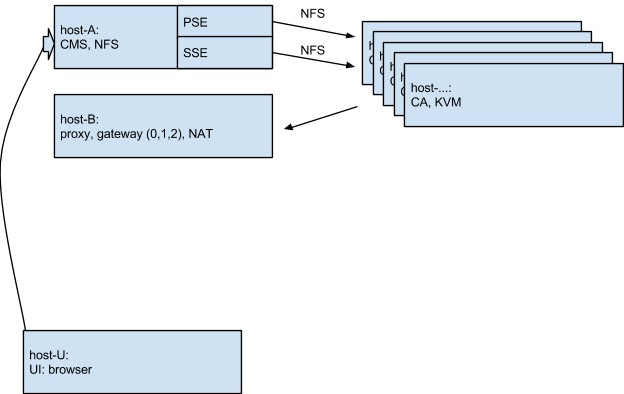
\includegraphics[width=\textwidth]{figures/hosts}
	\end{center}
	\caption{Hosts.}
	\label{fig:hardware:hosts}
\end{figure}



\section{Services Layout}
\label{sct:hardware:layout}
We recommend the following configuration:
\begin{description}
	\item[\host{A}] \acrshort{cms}, \acrshort{pse}, \acrshort{sse}
	\item[\host{B}] \acrshort{sq}, \acrshort{gwext}, \acrshort{gwint}
	\item[\host{C}, \host{D}, \dots] \acrshort{ca}
	\item[\host{U}] Administrator/User computer
\end{description}

\begin{figure}
	\begin{center}
		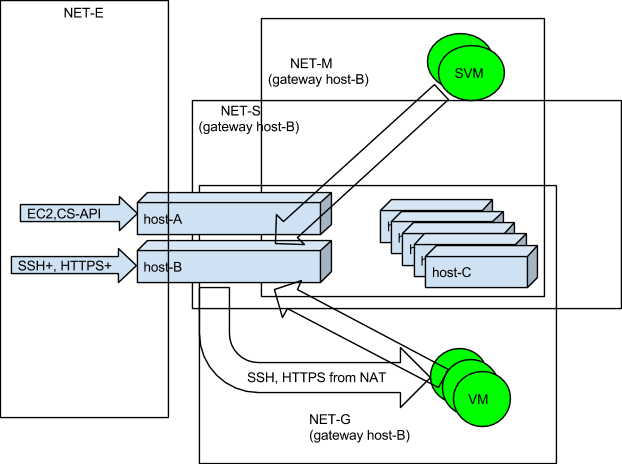
\includegraphics[width=\textwidth]{figures/layout}
	\end{center}
	\caption{Services layout.}
	\label{fig:hardware:layout}
\end{figure}

\section{Network Configuration}
\label{sct:hardware:network}

\subsection{Configuration via ``Basic Zone Network''}

If we are going to configure the network for \cstack\ using ``Basic Zone Network'', we need four preconfigured networks:
\begin{enumerate}
	\item \acrfull{nete}
	\item \acrfull{nets}
	\item \acrfull{netm}
	\item \acrfull{netg}
\end{enumerate}

\subsubsection{\acrfull{nete}}
External network is used for accessing to cloud through \acrshort{ec2api}, \acrshort{csapi} and selected virtual machines from internet/unsecured networks.
This network must be configured on \host{A} (for accessing to the \acrshort{ec2api} and \acrshort{csapi}) and on \host{B} (for access to virtual machines via \acrshort{nat}).

\subsubsection{\acrfull{nets}}
The storage network is used to provide access to storage pools for \acrshort{ca}s. 
It must be configured on \host{A} and on \acrshort{ca}s hosts (\host{C}, \host{D}, \dots).

\subsubsection{\acrfull{netm}}
The management network is used for communication between the \cstack\ components. 
All hosts must be able to connect to this network.

\subsubsection{\acrfull{netg}}
The guest network is used for communication between virtual machines and between virtual machines and external network, also it used for \acrshort{nat}-ing ports 22 and 443 to the external network.
\acrshort{netg} \acrshort{nat} rules must be configured on \host{B}.
At present time we use the following rules for port forwarding
\begin{lstlisting}
-A PREROUTING -d host-B -p tcp -m tcp --dport x443 -j DNAT --to-destination 10.1.2.x:443
-A PREROUTING -d host-B -p tcp -m tcp --dport x022 -j DNAT --to-destination 10.1.2.x:22
\end{lstlisting}
10.1.2.x is an IP of a virtual machine in \acrshort{netg}.

\chapter{\cstack\ Installation}
\label{cpt:cloudstack}


\section{\acrlong{cms}}
\label{sct:cloudstack:cms}

It is recommended to install \cstack\ on CentOS~6.4 or higher.
During installation process we will need the following shell variables:
\begin{lstlisting}
MYSQLPASSWD
USERCLOUD
PASSWDCLOUD
\end{lstlisting}
Add the repository:
\begin{lstlisting}
cat >> /etc/yum.repos.d/cloudstack.repo << EOF
[cloudstack]
name=cloudstack
baseurl=http://cloudstack.apt-get.eu/rhel/4.2/
enabled=1
gpgcheck=0
EOF
\end{lstlisting}
Install packages:
\begin{lstlisting}
yum -y install ntp mysql-server cloudstack-management wget
\end{lstlisting}
Perform additional configuration:
\begin{lstlisting}
setenforce 0
sed s/"SELINUX=.*"/"SELINUX=permissive"/g -i /etc/selinux/config
ntpdate 0.centos.pool.ntp.org
service ntpd start
chkconfig ntpd on
mv /etc/my.cnf /etc/my.cnf.save
echo "
[mysqld]
datadir=/var/lib/mysql
socket=/var/lib/mysql/mysql.sock
user=mysql
# Disabling symbolic-links is recommended to prevent assorted security risks
symbolic-links=0

innodb_rollback_on_timeout=1
innodb_lock_wait_timeout=600
max_connections=700
log-bin=mysql-bin
binlog-format = 'ROW'
bind-address = 0.0.0.0
[mysqld_safe]
log-error=/var/log/mysqld.log
pid-file=/var/run/mysqld/mysqld.pid
" > /etc/my.cnf
service mysqld start
mysqladmin -u root password $MYSQLPASSWD
mysqladmin -u root -h $hostname  password $MYSQLPASSWD
chkconfig mysqld on
service mysql restart
\end{lstlisting}
CloudStack database setup:
\begin{lstlisting}
cloudstack-setup-databases $USERCLOUD:$PASSWDCLOUD@localhost \
  --deploy-as=root:$MYSQLPASSWD
\end{lstlisting}

If one is going to use HTTPS for connection to \acrshort{ec2api} and \acrshort{csapi}, it is required to use \cstack\ 4.4 or newer or to patch \cstack\ manually\footnote{\url{https://reviews.apache.org/r/17586}}.
Otherwise only HTTP configuration of \cstack\ will work correctly.
Configure \cstack\ for HTTPS:
\begin{lstlisting}
cloudstack-setup-management --https
\end{lstlisting}
Check configuration file /etc/cloudstack/management/ec2-service.properties:
\begin{lstlisting}
managementServer=127.0.0.1
cloudAPIPort=6443
cloudAPISSLEnabled=true
cloudstackVersion=2.2.0
WSDLVersion=2012-08-15
keystore=xes.keystore
keystorePass=apache
\end{lstlisting}
Option \texttt{cloudAPISSLEnabled=true} is available only for patched version of \cstack.
After this configuration is performed, it is highly recommended to change password (see Section~\ref{sct:config:passwd}). 
Also do not open ports to external network before changing password.


\section{\acrlong{ca}}
\label{sct:cloudstack:ca}

It is recommended to install \cstack\ on CentOS~6.4 or higher.
Add repository:
\begin{lstlisting}
cat  >>  /etc/yum.repos.d/cloudstack.repo << EOF
[cloudstack]
name=cloudstack
baseurl=http://cloudstack.apt-get.eu/rhel/4.2/
enabled=1
gpgcheck=0
EOF
\end{lstlisting}
Install packages:
\begin{lstlisting}
yum -y install ntp cloudstack-agent libvirt-client  qemu-kvm virt-manager
\end{lstlisting}
Perform additional configuration:
\begin{lstlisting}
setenforce 0
sed s/"SELINUX=.*"/"SELINUX=permissive"/g -i  /etc/selinux/config
ntpdate 0.centos.pool.ntp.org
service ntpd start
chkconfig ntpd on
sed s/"listen_tls.*"/"listen_tls = 0"/g -i /etc/libvirt/libvirtd.conf
sed s/"listen_tcp.*"/"listen_tcp = 1"/g -i /etc/libvirt/libvirtd.conf
sed s/"tcp_port.*"/"tcp_port = 16509"/g -i /etc/libvirt/libvirtd.conf
sed s/"auth_tcp.*"/"auth_tcp = \"none\""/g -i /etc/libvirt/libvirtd.conf
sed s/"mdns_adv.*"/"mdns_adv = 0"/g -i /etc/libvirt/libvirtd.conf
echo "LIBVIRTD_ARGS=--listen" >> /etc/sysconfig/libvirtd
service libvirtd restart
\end{lstlisting}


\section{Storage Engine}
One must configure an NFS server accessible from \acrshort{nets} and provide to folders for \acrshort{pse} and \acrshort{sse}.
In /etc/sysconfig/nfs uncomment the following lines:
\begin{lstlisting}
LOCKD_TCPPORT=32803
LOCKD_UDPPORT=32769
MOUNTD_PORT=892
RQUOTAD_PORT=875
STATD_PORT=662
STATD_OUTGOING_PORT=2020
\end{lstlisting}

To perform the next step one need access to \acrshort{sse} from \acrshort{cms} (in the configuration under consideration this takes place, otherwise one needs to mount \acrshort{sse} share on \acrshort{cms} to some folder, for example \texttt{\$DIR}).  
\texttt{\$DIR} is the location of \acrshort{sse} folder on \acrshort{cms}.
Now one need to execute the following command (please consult the \cstack\ guide for proper template name\footnote{\url{http://docs.cloudstack.apache.org/projects/cloudstack-installation/en/latest/installation.html\#prepare-the-system-vm-template}})
\begin{lstlisting}
 /usr/share/cloudstack-common/scripts/storage/secondary/cloud-install-sys-tmplt -m $DIR \
   -u http://d21ifhcun6b1t2.cloudfront.net/templates/4.2/systemvmtemplate-2013-06-12-master-kvm.qcow2.bz2 \
   -h kvm -F
\end{lstlisting}

\chapter{CloudStack Configuration and First Launch}
\label{cpt:config}

\section{Changing the Root Password}
\label{sct:config:passwd}

Following CloudStack documentation:
\begin{quote}
	During installation and ongoing cloud administration, you will need to log in to the UI as the root administrator. 
	The root administrator account manages the CloudStack deployment, including physical infrastructure. 
	The root administrator can modify configuration settings to change basic functionality, create or delete user accounts, and take many actions that should be performed only by an authorized person. 
	When first installing CloudStack, be sure to change the default password to a new, unique value.
	\begin{enumerate}
		\item Open your favorite Web browser and go to this URL.
			Substitute the IP address of your own Management Server:\\
			\url{https://<management-server-ip-address>:6443/client}
		\item Log in to the UI using the current root user ID and password. 
			The default is admin, password.
		\item Click Accounts.
		\item Click the admin account name.
		\item Click View Users.
		\item Click the admin user name.
		\item Click the Change Password button. 
\includegraphics[height=2ex]{figures/passwd}
		\item Type the new password, and click OK.
	\end{enumerate}
\end{quote}


\section{Adding Users and Keys}
\label{sct:config:accounts}

At least two users are required for standard \cstack\ configuration: administrator (default name admin) and non-privileged user.
Moreover in order to use \acrshort{csapi} or \acrshort{ec2api} one needs authorization keys. 
At first step we will create administrators keys following \cstack\ documentation:
\begin{quote}
	\begin{enumerate}
		\item Open your favorite Web browser and go to this URL.
			Substitute the IP address of your own Management Server:\\
			\url{https://<management-server-ip-address>:6443/client}
		\item Log in to the UI using the current root user ID and password. 
		\item Click Accounts.
		\item Click the admin account name.
		\item Click View Users.
		\item Click ``Generate keys''
		\item Click ``Yes''
		\item Copy API Key and Secret Key for future.
	\end{enumerate}
\end{quote}

Now we are able to use \acrshort{csapi}\footnote{\url{http://cloudstack.apache.org/docs/api}}.
Now let us create non-privileged user \emph{cvmuser} with account type ``User''.
\begin{quote}
	\begin{enumerate}
		\item Open your favorite Web browser and go to this URL.
			Substitute the IP address of your own Management Server:\\
			\url{https://<management-server-ip-address>:6443/client}
		\item Log in to the UI using the current root user ID and password. 
		\item Click Accounts.
		\item Click ``add accounts''
		\item Fill all fields and set Account type to User.
		\item Create user keys in the same way as for admin user.
	\end{enumerate}
\end{quote}


\section{Setting Global Variables}
\label{sct:config:globalvars}

For our particular task (launching \cernvm\ based elastic clusters) we need to change a number of global variables:
\begin{quote}
	\begin{enumerate}
		\item Open your favorite Web browser and go to this URL.
			Substitute the IP address of your own Management Server:\\
			\url{https://<management-server-ip-address>:6443/client}
		\item Log in to the UI using the current root user ID and password. 
		\item Click Global Settings
		\item Use find field to locate variables.
	\end{enumerate}
\end{quote}
Variables to be tuned:
\begin{lstlisting}[deletekeywords={true,enable}]
host                         "real host IP"  # example 195.19.226.152
management.network.cidr      "real cidr"     # example 195.19.226.129/27
expunge.delay                60
expunge.interval             60
expunge.workers              1               # usually you don't need more than one worker
max.account.primary.storage  400             # quota of primary storage for user in Gb,
                                             # depends on size of your storage
max.project.primary.storage  400             # quota of primary storage for project in Gb,
                                             # depends on size of your storage
enable.ec2.api               true
\end{lstlisting}
Now one need to restart \acrshort{cms} service on \host{A}:
\begin{lstlisting}
service cloudstack-management restart
\end{lstlisting}


\section{Enabling \acrshort{ec2api}}
For correct operation of \cernvm\ and elastic clusters one needs \acrshort{ec2api} configured.
To configure \acrshort{ec2api} global variable, \texttt{enable.ec2.api} must be set to true (see Section~\ref{sct:config:globalvars}). 
API access keys (see Section~\ref{sct:config:accounts}), private key and self-signed X.509 certificate are also required.
\begin{lstlisting}
EC2_AKEY="..."
EC2_SKEY="..."
cloudstack-aws-api-register --apikey=$EC2_AKEY --secretkey=$EC2_SKEY \
  --cert=~/.globus/usercert.pem --url=https://alice22.spbu.ru:5443/awsapi/
\end{lstlisting}


\section{Zone Creation, Adding Storages and Hosts}

Using web-interface.
\begin{enumerate}
	\item Open your favorite Web browser and go to this URL.
		Substitute the IP address of your own Management Server:\\
		\url{https://<management-server-ip-address>:6443/client}
	\item Log in to the UI using the current root user ID and password. 
		The default is admin, password
	\item Click Infrastructure
	\item Click add Zone
	\item Step by step create zone
	\begin{enumerate}
		\item type BASIC
		\item Hypervisor -- KVM
		\item Pod network -- \acrfull{netm}
		\item Guest network -- \acrshort{netg}. 
			\emph{\acrshort{netg} and \acrshort{netm} must be different!}
		\item host add -- put root username and  password
		\item Secondary storage provider -- NFS
	\end{enumerate}
\end{enumerate}

\chapter{Known issues with CernVM on CloudStack}
\label{cpt:issues}

\section{Downloading and Configuring Image}
One can download \cernvm\ from \url{http://cernvm.cern.ch/portal/downloads}.
\cstack\ supports QCOW2, RAW, and VHD formats. 
\cstack\ offerings available from \acrshort{ec2api} does not include disk offerings. 
In order to lunch \cernvm\ correctly one need to enlarge \cernvm\ image up to size required for \cernvm\ instances.

\begin{lstlisting}[deletekeywords={if}]
dd if=/dev/zero of=~/20GB bs=1M count=20000
qemu-img convert -O qcow2 ucernvm-devel.1.15-7.cernvm.2G2.x86_64.qcow2 \
  ~/20GB ucernvm-devel.1.15-7.cernvm-2G.x86_64.qcow2
\end{lstlisting}
Resulting file must be uploaded to some HTTP server.
And after that upload it to \cstack\ using web interface


\section{Configuring CloudStack for CernVM}

\subsection{Compute Offerings}
\acrshort{ec2api} has standard default names for Compute Offerings\footnote{\url{http://aws.amazon.com/ec2/instance-types/\#instance-details}}, so it is suitable to create \cstack\ Compute Offerings m1.medium and m1.small in ``Service Offerings'' $\rightarrow$ ``Compute Offerings'' web-interface section.

\subsection{defaultGuestNetwork configuration}
For normal operation \cernvm\ requires additional tuning of networks
\begin{itemize}
	\item it requires access to 22 and 443 ports for head node
	\item and non-firewalled network between nodes (for condor)
\end{itemize}
One can configure it using web-interface in Network $\rightarrow$ Security Groups section from \emph{cvmuser} account.
Edit \emph{default} security group, add to ``Ingress rule''  the following rules:
\begin{lstlisting}
Protocol    Start Port    End Port    CIDR
TCP         22            22          0.0.0.0/0
TCP         443           443         0.0.0.0/0
TCP         1024          60000       10.1.2.0/24
\end{lstlisting}
Where 10.1.2.0/24 is \acrshort{netg}. 


\section{User-data}
While creating user-data (for example, using \url{https://cernvm-online.cern.ch}) one needs to take into account the following:
\begin{itemize}
	\item \acrshort{ec2api} version must be set equal to version in /etc/cloudstack/management/ec2-service.properties on \acrshort{cms} (\host{A})
	\item \acrshort{ec2api} URL -- address of  \acrshort{ec2api} of your cloud (\eg \url{https://HOST-A-internal:5443/awsapi})
	\item EC2 Image AMI ID - must be set to  imageID, not image name
	\item Proxy -- your internal proxy.
	\item To allow elastiq to work correctly with self-signed certificates one need to add to user data the following script:
	\begin{lstlisting}
echo '[Boto]
https_validate_certificates = False' >> /var/lib/condor/.boto
chown condor: /var/lib/condor/.boto
service elastiq restart
	\end{lstlisting}
	This solution may be considered as good enough, because it is assumed that master node communicates with cloud via isolated network. 
	In general it is better to add your certificate authority to boto.
\end{itemize}


\section{CernVM Deployment}
For deploying \cernvm instances we use scripts from Appendix~\ref{apx:scripts}. 
These scripts are analogous to scripts from euca-tools, but written using boto and able to change \acrshort{ec2api} version (which is necessary for \cstack).
To launch an instance one needs to set bash variables with access keys, url and \acrshort{ec2api} version (see Appendix~\ref{apx:scripts}) and run the following script:
\begin{lstlisting}
./uni-run-instances.py -t m1.medium -k 'lxkey' -d "
[amiconfig]
plugins=cernvm
[cernvm]
contextualization_key=521b58d9e5274b0c803aadf71520cb17
[ucernvm-begin]
resize_rootfs=true
cvmfs_branch=cernvm-devel.cern.ch
cvmfs_server=hepvm.cern.ch
[ucernvm-end]" cernvm3
\end{lstlisting}


\appendix
\chapter{Scripts}
\label{apx:scripts}


\section{uni-list-instances.py}
This script prints list of users virtual machines.
The output of the script contains the following information: DNS\_NAME ``dns name of VM(if exists)''  ID\_ADR ``VM's ip address'' ID ``VM's id'' STATUS ``VM's status (running, stopped, etc.)''
For operating script requires the following shell variables to be set:
\begin{lstlisting}
# users ec2 access key:
EC2_ACCESS_KEY 
# users ec2 secret key:
EC2_SECRET_KEY
# cloud ec2 url:
EC2_URL
# ec2 api version supported by this cloud:
EC2_API_VERSION
\end{lstlisting}
The last variable is set by default to 2012-08-15.
Sample script for setting up variables can be found at \url{http://alice03.spbu.ru/soft/boto-scripts/ec2en.sh}

\noindent Example:
\begin{lstlisting}
./uni-list-instances.py
DNS_NAME  ID_ADR 10.1.2.9 ID 27c1fbb1-6fda-4a19-bcfb-d0c0b2254600 STATUS running
DNS_NAME  ID_ADR 10.1.2.8 ID b0771bc4-8a2d-48de-9f01-1e03ce8b9b9b STATUS running
\end{lstlisting}
Location: \url{http://alice03.spbu.ru/soft/boto-scripts/uni-list-instances.py}


\section{uni-run-instances.py}
Script deploys virtual machine with given options into cloud.\\
Options: \texttt{./uni-run-instances.py  -t ``Instance Type'' -k ``name of ssh key'' -d ``user data (text format)'' ``image id''}\\
The output of the script contains the following information: RESERVATION    ``reservation id''    ``owner id''    ``security group'' INSTANCE        ``instance id''      ``image id''    ``private dns name''     ``instance state''  ``ssh key name''   ``launch index''       ``instance type''      ``launch time''  ``placement''    ``monitoring state''    ``dns name'' ``root device type''

For operating script requires the following shell variables to be set:
\begin{lstlisting}
# users ec2 access key:
EC2_ACCESS_KEY 
# users ec2 secret key:
EC2_SECRET_KEY
# cloud ec2 url:
EC2_URL
# ec2 api version supported by this cloud:
EC2_API_VERSION
\end{lstlisting}
The last variable is set by default to 2012-08-15.

\noindent Example:
\begin{lstlisting}
./uni-run-instances.py  -t m1.medium -k 'lxkey' -d "
[amiconfig]
plugins=cernvm
[cernvm]
contextualization_key=521b58d9e5274b0c803aadf71520cb17
[ucernvm-begin]
resize_rootfs=true
cvmfs_branch=cernvm-devel.cern.ch
cvmfs_server=hepvm.cern.ch
[ucernvm-end]"  cernvm3
RESERVATION     r-gjia2vsg      de985467-75d6-466e-829c-be6273c3c952    default
INSTANCE        i-0001f0a1      ami-0000025f    ...
\end{lstlisting}
Location: \url{http://alice03.spbu.ru/soft/boto-scripts/uni-run-instances.py}



%\pagestyle{plain}
%\bibliographystyle{alpha}
%\bibliography{references}

%\printindex

\end{document}
